As described in \autoref{sec:architectures-attention}, the transformer architecture's performance can be improved by providing  \emph{positional encoding} (pe) information.
While with convolutions and pooling identical patches at different locations can be distinguished, in the attention mechanism they can not.
Adding pe resolves this issue.

The question arises, whether the \emph{masked} attention, that uses the graph information to confine the transformer to only its local neighborhood, also requires pe or not. 
Additionally if efficient training requires pe, it needs to be discussed what type works best.

\begin{figure}[htbp]
    \centering
    \makebox[\textwidth][c]{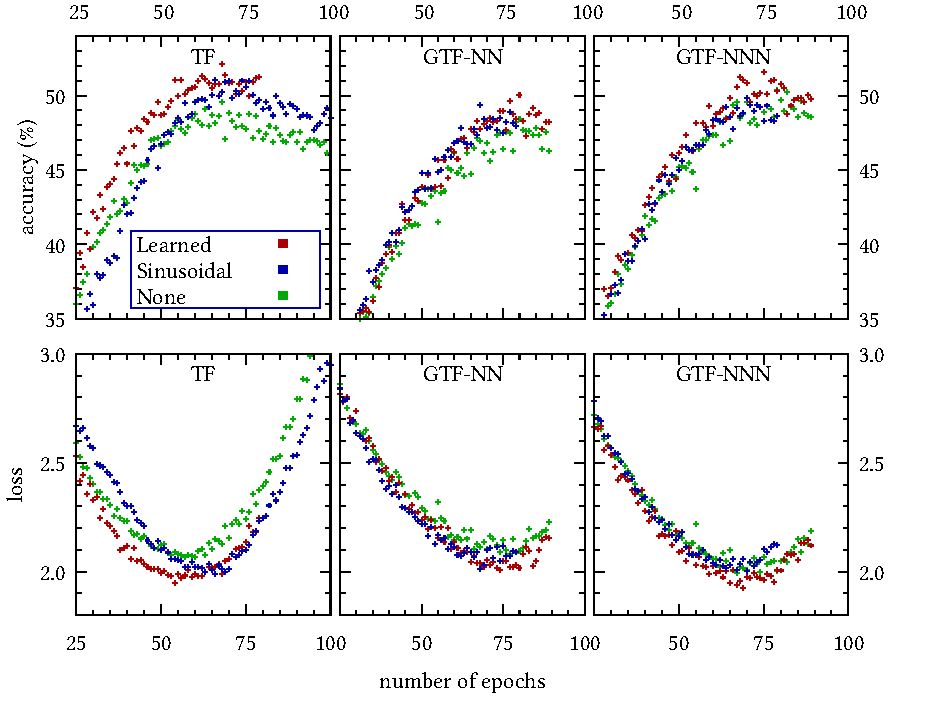
\includegraphics[width=1.1\textwidth]{./experiments/image-classification/positional-encoding/pe-comparison/pe-comparison.pdf}}
    \caption{Visualization of the training attention and loss metrics for three different models. \emph{TF}, \emph{GTF-NN} and \emph{GTF-NNN}.
    Only part of the full training is shown. 
    Each model was trained once with \emph{sinusoidal} pe, \emph{learned} pe and \emph{without} any additional pe.
    Apart from that all hyperparameters are kept static.
    }
    \label{fig:positional-encoding-training}
\end{figure}

The simulations are visualized in \autoref{fig:positional-encoding-training}.
It can be seen, that the different architectures react differently to the types of pe.

The data clearly shows benefits in employing pe. 
All models show an increase in accuracy of about \SIrange[]{3}{4}{\percent}. 
This is less than the difference between some of the other token mixing elements, but still a significant margin in comparison to the absolute performance.
As adding pe is rather cheap, the employment of this strategy can definitely be useful:
Both types of pe are only added at the start of the calculation.
Therefore the cost is not dependent on the depth or type of token-mixer.
Calculating sinusoidal pe can theoretically be done once and the result can be cached, rendering it basically instantaneous to employ and of no negative computational impact. Furthermore it is resolution independent, as the sinus curves can later be sampled with a smaller interval in order to increase network resolution retrospectively.
Learned sinusoidal encodings on the other hand require a backwards propagation of error values into the encoding weights.
This requires additional computation and storage space, as well as providing no obvious way to update the encoding resolution after the fact.

The pure transformer definitely performs best with a learned pe. 
Not only is the overall accuracy higher ($\approx \SI[]{1.5}[]{\percent}$), but also is the loss-minimum reached about 12 epochs earlier - a huge potential reduction in necessary computation.

The GTF-NN model shows less benefit from applying pe.
This makes sense, as by design the number of attention targets is intentionally very limited. 
Sinusoidal pe and learned pe perform very similar, with sinusoidal pe converging ever so slightly faster than learned.
It should be noted though, that the sample size is too limited to draw definite conclusions from this tiny difference.

For the GTF-NNN the learned pe outperforms the sinusoidal one, taking about 5 epochs longer to converge, but accomplishing an about \SI[]{2}{\percent} higher accuracy.

To summarize, pe can definitely improve the performance of an attention based neural network. 
The correlation can hold true not only for normal attention as already know \cite{attentionIsAllYouNeed, imageWorth16x16}, but also for the attention mechanism with graph-limited influence, as the calculations demonstrate.

A challenge in more complex graph structures is undoubtably the definition of suitable pes, as the canonical sinusoidal encoding is not  extendable to irregular graphs.
The learned pe would probably constitute the easiest and best solution, but comes with a computational overhead both in terms of the cost of one epoch, as well as the speed of convergence, i.e. the needed number of epochs until the calculation converges.

In the ground state search task, no positional encoding is applied. 
Its application could be a task for future research, especially on highly irregular graphs.